\chapter{Concurrency and Threads in .NET}
TODO: Chapter introduction

\section{Concurrency terminology}
This section defines common terminology used in this thesis. These terms are often used in the same context, but even though they are similar, they have different meanings. It is imperative to be aware of these distinctions in order to be able to reason clearly about software and multithreading.

\subsubsection{Sequential programming}
\emph{Sequential programming} is a way of writing code as step by step instructions. It is a convenient and easy to understand approach where mistakes about what to do and when do it are less common.
The disadvantage of performing operations this way is that the thread must wait during parts of the process, being effectively blocked. Blocking threads and singular instructions make poor use of device resources.
To reiterate, sequential programming is a set of consecutive, progressively ordered instruction execution in linear fashion (fig. \ref{fig:seq}).

\begin{figure}[ht!]
	\centering
		
\includegraphics[width=\columnwidth]{figures02/seq.png}
	\caption{Sequential programming involves executing progressively ordered set of instructions}
	\label{fig:seq}
\end{figure}

In imperative and object-oriented languages there is a tendency to write sequential code, with all attention and resources focused on the task currently running. Programs are modeled and executed by performing an ordered set of statements, one after another. \cite{terrell_2018}

\subsubsection{Concurrent programming}
In computer science, \emph{concurrency} is the ability of different parts of a program, algorithm, or problem to be executed out-of-order or in partial order, without affecting the final outcome. \cite{lamport1978time}
\\ \\ 
Concurrency is used to achieve real multitasking in an application, by modeling the application into multiple, autonomous processes that run at the same in different threads.
As an example let's examine an online video streamer. The program downloads data from the network, decompresses it and displays the video on screen.
Concurrency gives the impression that all of these parts of the program are executing simultaneously, an illusion of parallelism is created. 
But in a single-core environment, the execution of one thread is temporarily paused and switched to another thread, this is called context switching, as shown in fig. \ref{fig:convspar}

\begin{figure}[ht!]
	\centering
		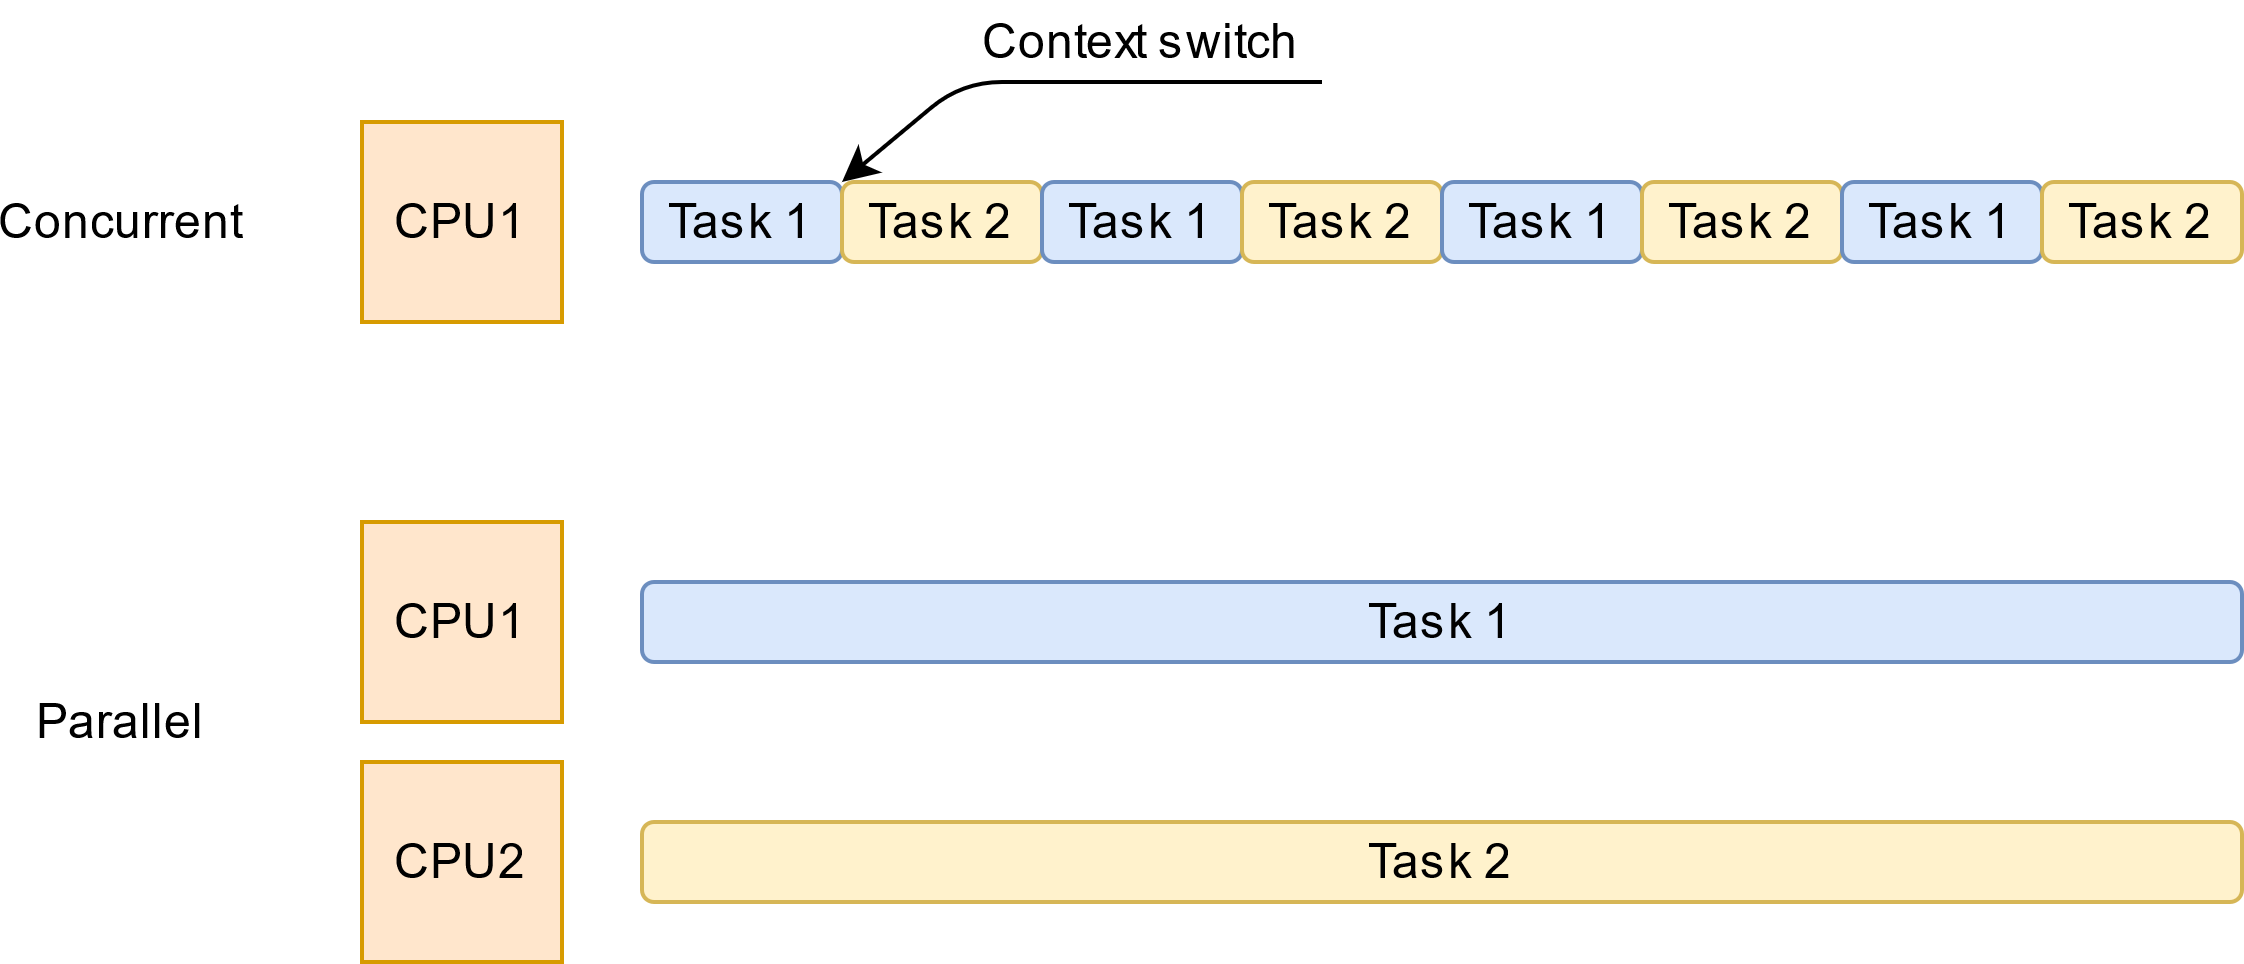
\includegraphics[width=\columnwidth]{figures02/convspar.png}
	\caption{Difference between concurrent and parallel models, both may look identical to the user}
	\label{fig:convspar}
\end{figure}

Concurrency is often confused with parallelism \cite{waza}, but concurrent programs only \emph{may} be executed in parallel 
by assigning each process to a separate processor or processor core, or distributing a computation across a network \cite{mordechai}

\subsubsection{Parallel programming}
\emph{Parallelism} is the idea of processing tasks simultaneously for performance and throughput improvement of a program. Although all parallel programs are concurrent, it was demonstrated that not all concurrency is parallel.
Parallel execution is constrained by the runtime environment of the program, devices need to be equiped with multicore CPUs to support it (fig.\ref{fig:convspar}).
\\ \\ 
Timing is the qualifying factor for parallelism. It may be achieved by dividing a single task into multiple, self-contained subtasks. When they are run simultaneously on available cores and their execution overlaps in time then the program is parallel (fig. \ref{fig:seqvspar}).

\begin{figure}[ht!]
	\centering
		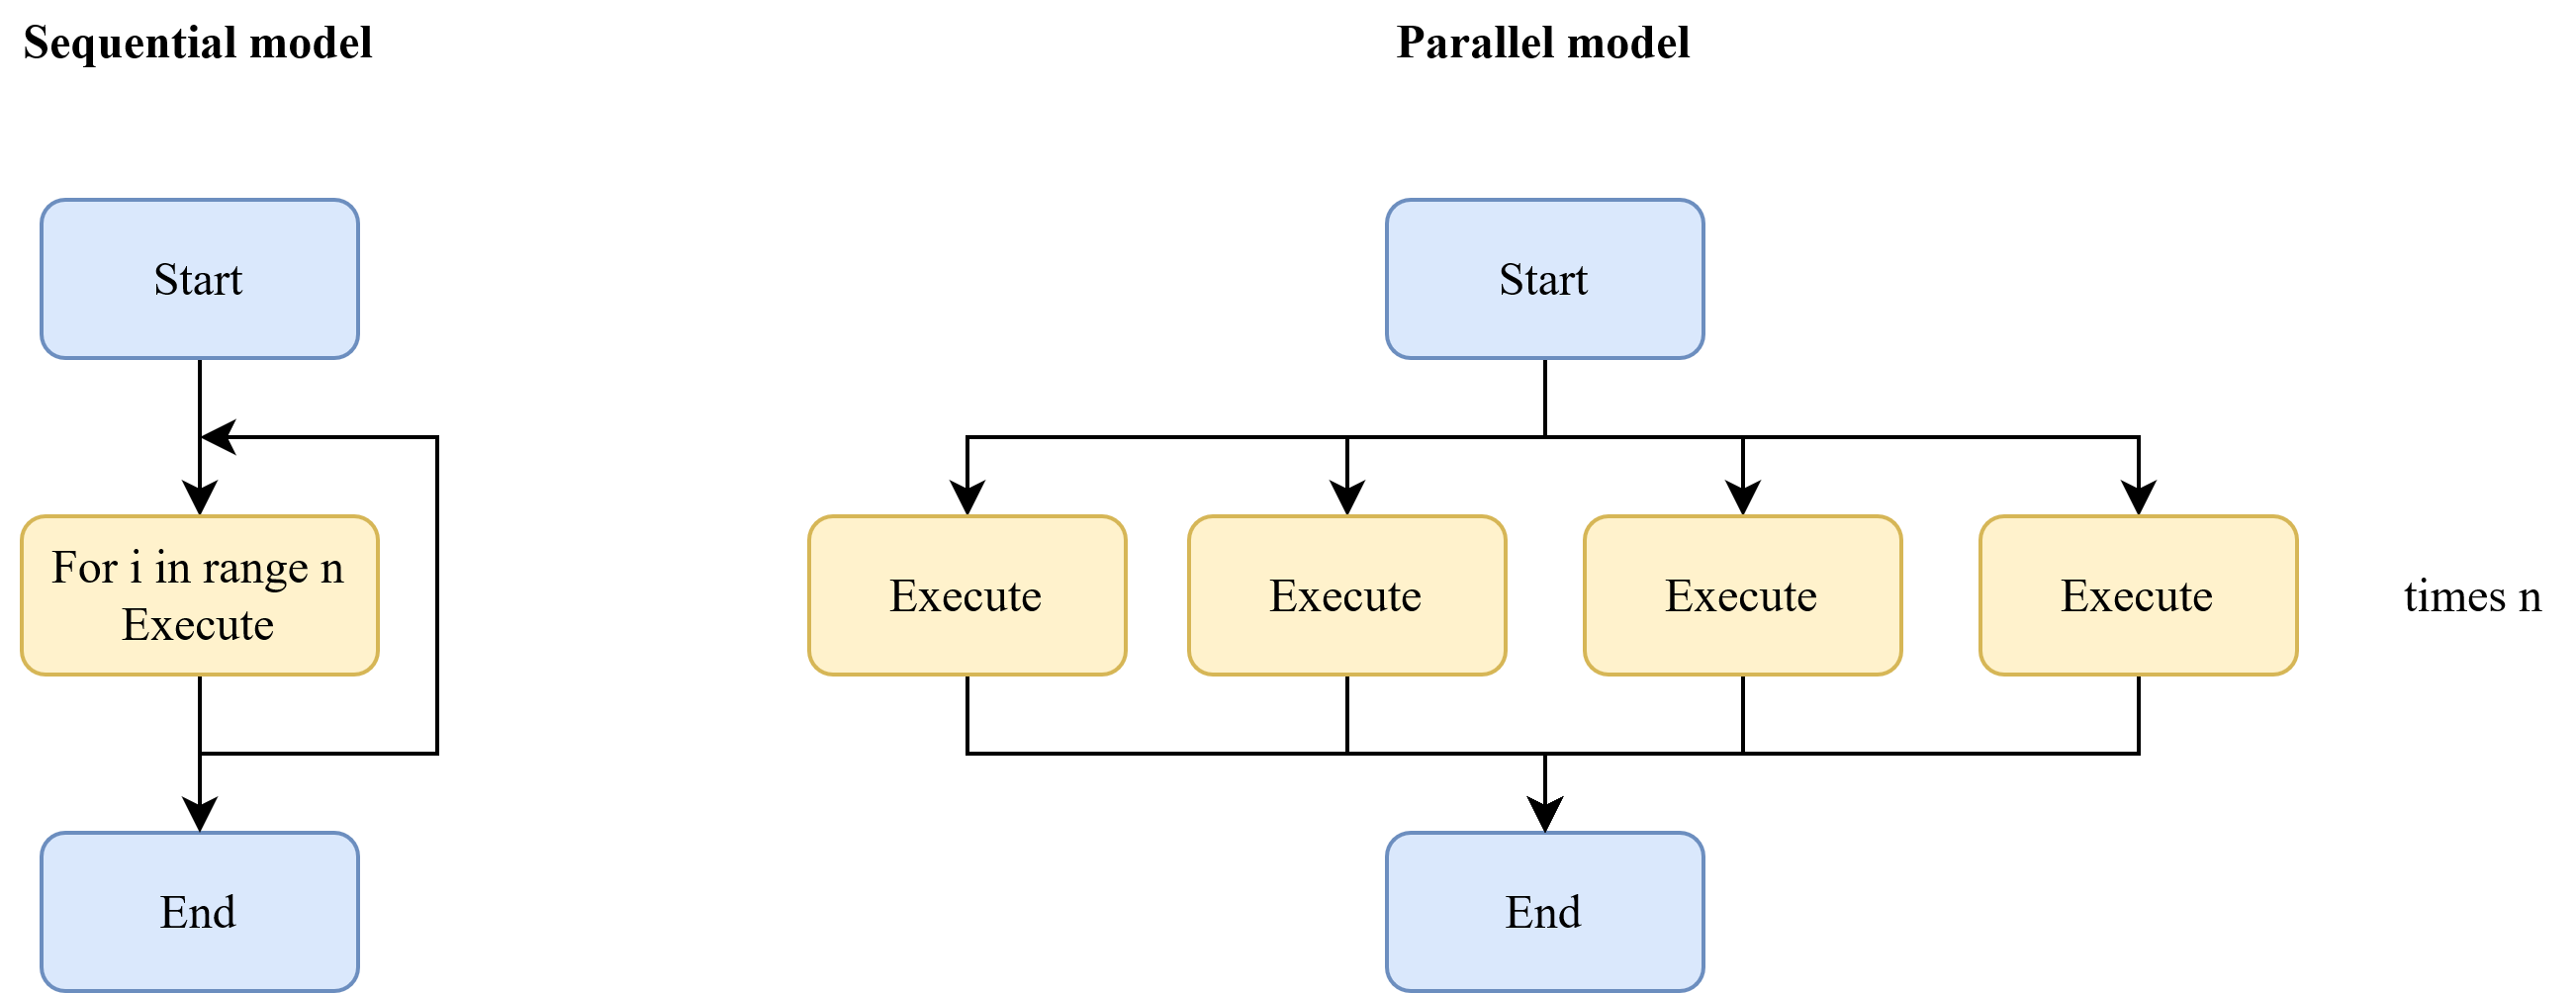
\includegraphics[width=\columnwidth]{figures02/seqvspar.png}
		\caption{Comparison of sequential and parallel models}
	\label{fig:seqvspar}
\end{figure}

\subsubsection{Multitasking}


Multitasking is the concept of performing multiple tasks over a period of time by executing
them concurrently. We�re familiar with this idea because we multitask all the
time in our daily lives. For example, while waiting for the barista to prepare our cappuccino,
we use our smartphone to check our emails or scan a news story. We�re doing
two things at one time: waiting and using a smartphone.
Computer multitasking was designed in the days when computers had a single CPU
to concurrently perform many tasks while sharing the same computing resources. Initially,
only one task could be executed at a time through time slicing of the CPU. (Time
slice refers to a sophisticated scheduling logic that coordinates execution between multiple
threads.) The amount of time the schedule allows a thread to run before scheduling
a different thread is called thread quantum. The CPU is time sliced so that each
thread gets to perform one operation before the execution context is switched to
another thread. Context switching is a procedure handled by the operating system to
Let�s start with terminology 11
multitask for optimized performance (figure 1.7). But in a single-core computer, it�s
possible that multitasking can slow down the performance of a program by introducing
extra overhead for context switching between threads.
Context switching on
a single-core machine
Figure 1.7 Each task has a different shade, indicating that the context switch in a single-core machine
gives the illusion that multiple tasks run in parallel, but only one task is processed at a time.
There are two kinds of multitasking operating systems:
? Cooperative multitasking systems, where the scheduler lets each task run until it finishes
or explicitly yields execution control back to the scheduler
? Preemptive multitasking systems (such as Microsoft Windows), where the scheduler
prioritizes the execution of tasks, and the underlying system, considering the priority
of the tasks, switches the execution sequence once the time allocation is
completed by yielding control to other tasks
Most operating systems designed in the last decade have provided preemptive multitasking.
Multitasking is useful for UI responsiveness to help avoid freezing the UI
during long operations.
\subsection{Multithreading}
Multithreading is an extension of the concept of multitasking, aiming to improve
the performance of a program by maximizing and optimizing computer resources.
Multithreading is a form of concurrency that uses multiple threads of execution.
Multithreading implies concurrency, but concurrency doesn�t necessarily imply multithreading.
Multithreading enables an application to explicitly subdivide specific tasks
into individual threads that run in parallel within the same process.
NOTE A process is an instance of a program running within a computer system.
Each process has one or more threads of execution, and no thread can exist
outside a process.
A thread is a unit of computation (an independent set of programming instructions
designed to achieve a particular result), which the operating system scheduler independently
executes and manages. Multithreading differs from multitasking: unlike
multitasking, with multithreading the threads share resources. But this �sharing
resources� design presents more programming challenges than multitasking does. We
discuss the problem of sharing variables between threads later in this chapter in section
1.4.1.
12 chapter 1 Functional concurrency foundations
The concepts of parallel and multithreading programming are closely related. But
in contrast to parallelism, multithreading is hardware-agnostic, which means that it can
be performed regardless of the number of cores. Parallel programming is a superset
of multithreading. You could use multithreading to parallelize a program by sharing
resources in the same process, for example, but you could also parallelize a program by
executing the computation in multiple processes or even

\section{Concurrency and threads in .NET}
This section will introduce .NET, the subject platform of this thesis. While in-depth understanding of it's vast inner workings may be helpful, it is not necessary for comprehension of this paper. Thus only a brief overview of .NET and Common Language Runtime (CLR) will be presented, reserving most space for explanation of .NET's threading and parallel execution tools. For readers desiring deeper knowledge and insights into CLR concepts I highly recommend exhaustive book \emph{CLR via C\#} by Jefrrey Richter \cite{richter}.

\subsubsection{.NET and CLR}
\emph{.NET} is a free, open-source development platform developed by Microsoft that supports building and running cross-platform apps of many kinds like:
\begin{itemize}
	\item Web apps, web APIs, and microservices
	\item Desktop apps
	\item Serverless functions in the cloud
	\item Mobile apps
\end{itemize}

All applications have access to the same runtime, APIs and class library which are the core elements of the .NET platform.
\\ \\ 
\emph{CLR} is the foundational virtual machine component of .NET which implements the Virtual Execution System (VES) defined by Microsoft's Common Language Infrastructure (CLI). The runtime is an agent that provides a managed execution environment, supporting core services such as memory management, thread management, and remoting, while also enforcing strict type safety and other forms of code accuracy that promote security and robustness. \cite{IntroductionToNet}
\\ \\ 
The managed execution process starts with choosing one of Commong Language Specification (CLS) compliant compilers, most popular being C\#, F\# and Visual Basic. The compiler translates source code into Microsoft Intermediate Language (MSIL). In this form code is CPU-independent and before it is run it must be converted to native code, usually by just-in-time (JIT) compiler. This process is performed on demand at application run time, when the contents of an assembly are loaded and executed \cite{ManagedExecution}.
CLR execution model is presented on fig. \ref{fig:clr}.

\begin{figure}[ht!]
	\centering
		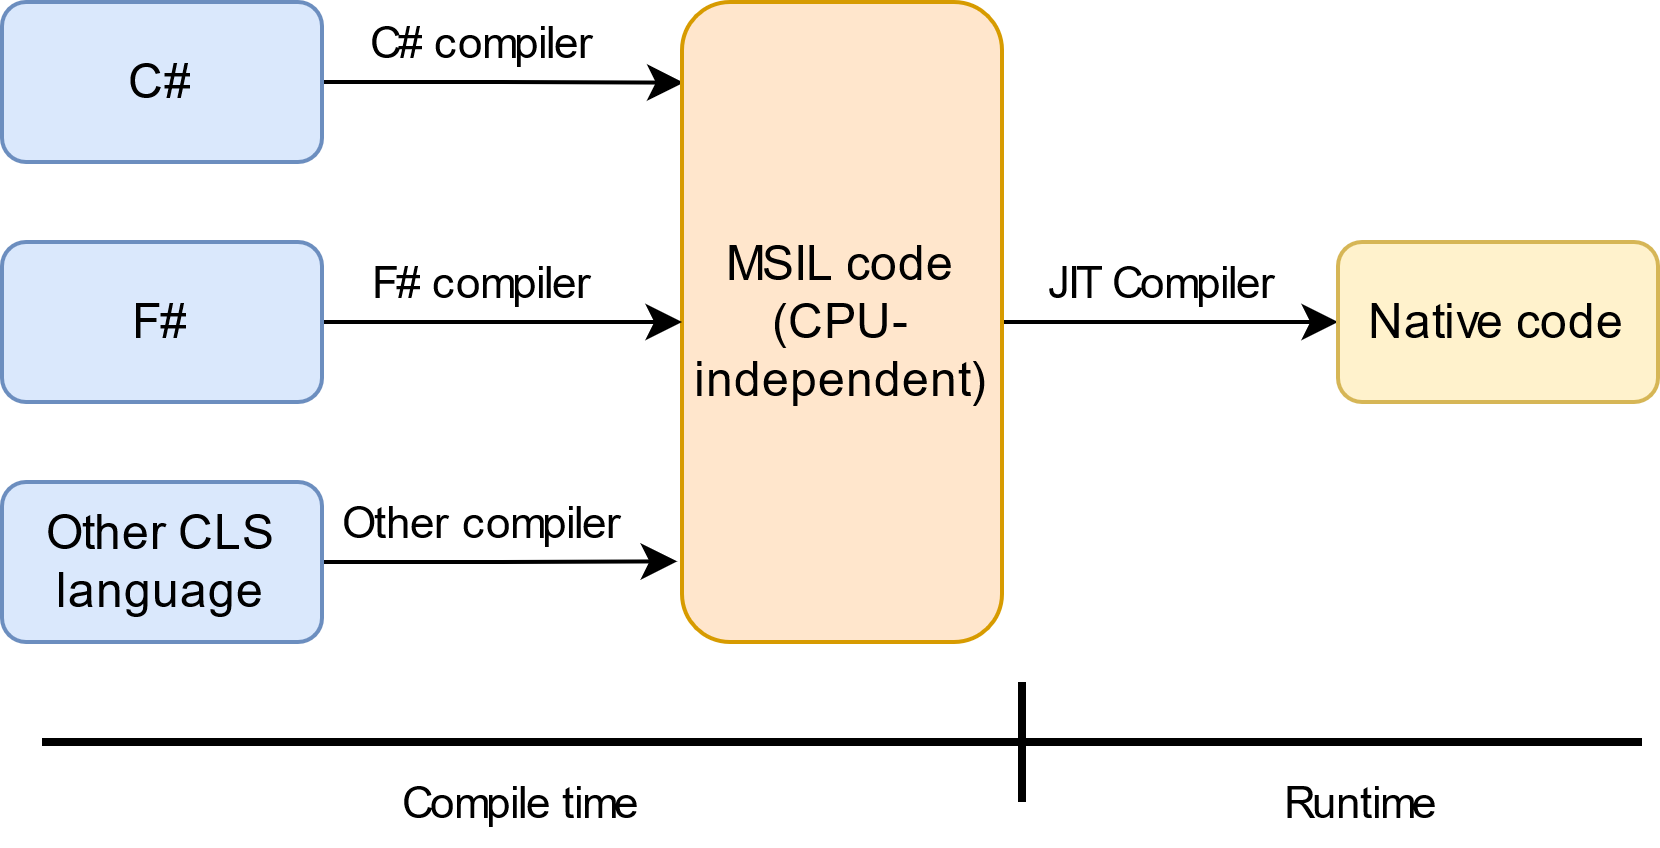
\includegraphics[width=0.8\columnwidth]{figures02/clr.png}
	\caption{CLR execution model}
	\label{fig:clr}
\end{figure}


\subsubsection{Threading in .NET}
A \emph{thread} is the fundamental unit to which an operating system (OS) allocates CPU time. Numerous threads can run inside of a \emph{process} which is a separate, executing program inside the OS.
When a thread is paused, system uses structures built into the thread to save it's context. The context contains all the information required for the thread to effortlessly resume execution. All threads spawned in the process share the same virtual address space and they can access and execute any part of the source code, including the parts currently handled by another thread. 
\\ \\ 
Most .NET programs start execution with a single thread, which is usually called the \emph{primary} thread. If the application requires parallel or asynchronous operations during runtime, additional threads, called \emph{worker threads} are created.
\\ \\ 
Management of all threads is done through the /emph{Thread} class, including threads created by the CLR and those created outside the runtime that enter the managed environment to execute code. The runtime monitors all the threads in its process that have ever executed code within the managed execution environment. It does not track any other threads.
\\ \\ 
A managed thread is either a \emph{background thread} or a \emph{foreground thread}. Foreground threads are what keeps the execution environment running. When all foreground threads in a managed process have been stopped, the system closes all background threads and shuts down the process.
\\ \\ 
Since all threads can accesses properties and methods of an single object, \emph{synchronization} is critical during multithreaded processing. Without it objects might me mutated into invalid state or threads might interrupt or even prevent each other from completing. A class whose members are protected from such interruptions is called \emph{thread-safe}. \cite{ManagedThreading} 
\\ \\ 
.NET provides several synchronization strategies including but not limited to:

\begin{itemize}
	\item Synchronized code regions with \emph{Monitor} class or compiler support.
	\item Manual synchronization with synchronization primitives.
	\item Collection classes in the System.Collections.Concurrent namespace. 
\end{itemize}

\subsubsection{Thread overhead}
Threads are a powerful tool which enable greater responsiveness and throughput of program, but as with every virtualization mechanism, threads have memory consumption and runtime execution performance overhead associated with them. That overhead will be later measured during experiments, so it's important to explore what's causing it. 
\\ \\
Creating, destroying and having threads existing in the system has time and space overhead since all threads has one of each of the following:
\begin{itemize}
	\item \textbf{Thread kernel object} -  data structure containing thread properties like CPU registers.
	\item \textbf{Thread environment block} -  block of memory which contains the head of the thread's exception handling chain.
	\item \textbf{User-mode stack} - stack used for local variables and method arguments.
	\item \textbf{Kernel-mode stack} - stack used for kernel-mode method arguments. Arguments are copied from user-mode stack to kernel-mode stack for security reasons.
	\item \textbf{DLL thread-attach and thread-detach notifications} - DLL\_THREAD\_ATTACH and DLL\_THREAD\_DETACH flags are passed to unmanaged DLLs when they are loaded by the process.
\end{itemize}

A CPU can only simultaneously execute as many threads as there are physical cores. Therefore, OS has to share the actual CPU hardware among all the threads (logical CPUs) that are sitting around in the system. In .NET a thread is allowed to run for a time-slice. When it expires, context switch occurs. Every context switch requires:

\begin{itemize}
	\item Saving the values of CPU's registers to the thread's kernel object
	\item Selecting another thread to schedule. If this thread belong to another process, then new virtual address space must be loaded.
	\item Load values of CPU's registers from the thread's kernel object
\end{itemize}

On top of that, if the new thread doesn't use the same code and data as the previous thread, then CPU has to access RAM memory to populate it's cache.
\\ \\ 
Context switches are needed to provide end users with responsive experience, but there is no other memory or performance benefit to them. Since they are pure overhead, they should be minimized when programming for performance. \cite{Richter2012Overhead}
   
\subsubsection{ThreadPool in CLR} 
To improve the resource consumption situation, the CLR contains code to manage its own ThreadPool. Instead of creating and deleting threads for every request, it maintains a set of threads for reuse. Tasks from operation queue are dispatched to threads existing in the pool. When the task is completed, thread is returned to the pool instead of being deleted (fig. \ref{fig:threadpool}).

\begin{figure}[!ht]
	\centering
		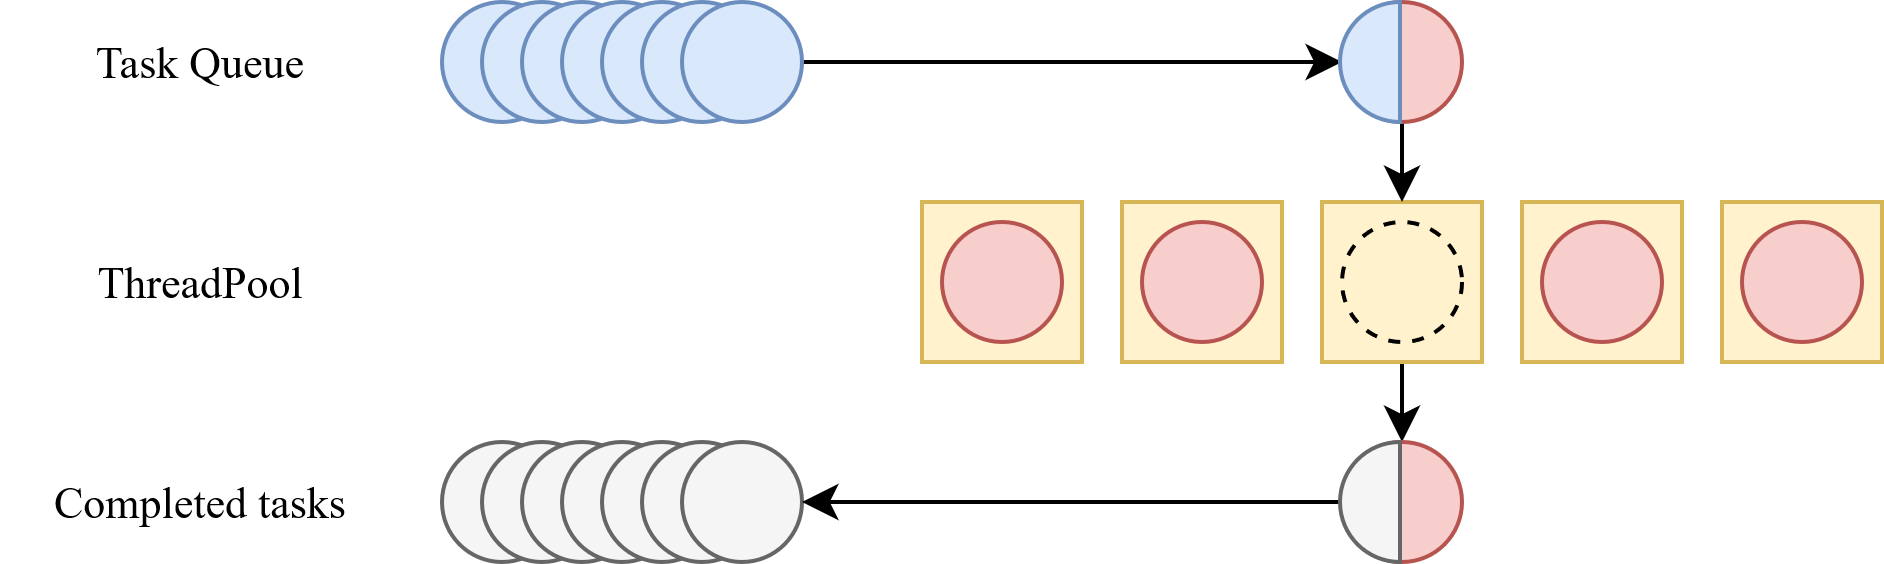
\includegraphics[width=0.8\columnwidth]{figures02/threadpool.png}
		\caption{Thread pool decreases resource consumption associated with creating and deleting threads}
		\label{fig:threadpool}
\end{figure}


CLR's ThreadPool saw many advancements in .NET 4.0 release, facilitating concurrent and parallel execution on multi-core architectures. Two major points were considered during development, quick work dispatch and throttling the degree of parallelism. While the former one is very important, it has relatively low impact on the topic of this paper. 
However, it is important to know that the CLR uses Hill Climbing (HC algorithm (fig. \ref{fig:hc}) and signal processing techniques to throttle the amount of threads spawned in the ThreadPool. These can, in specific and rare situations, be manually adjusted for further performance increases \cite{Fuentes2010}.

\begin{figure}[!ht]
	\centering
		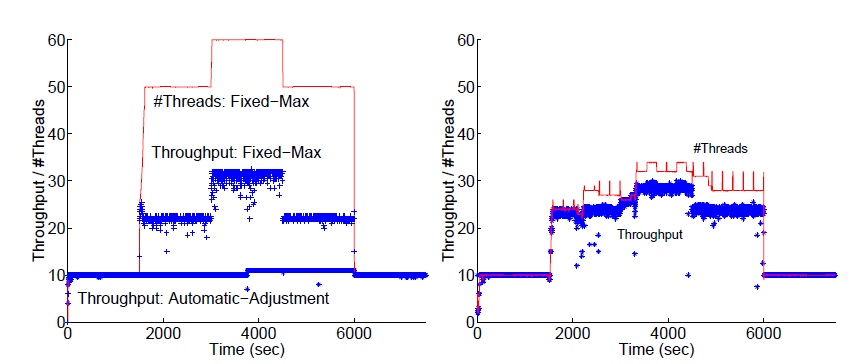
\includegraphics[width=0.8\columnwidth]{figures02/hc.PNG}
	\caption{Comparison of the old concurrency controller and .NET 4.0 HC concurrency controller \cite{Hellerstein2008}}
	\label{fig:hc}
\end{figure}

\subsubsection{Synchronization primitives}

\subsubsection{Concurrent collections}

\subsubsection{Parallel stuff}

